% Number 740
% Springs CoEM ETM Algebra Units Vectors
% springs - non-Hooke and CoEM, ETM
% JG

% Watermark
\AddToShipoutPicture*{\BackgroundPic}

\addtocounter {ProbNum} {1}

%\begin{floatingfigure}[r]{.42\textwidth}
%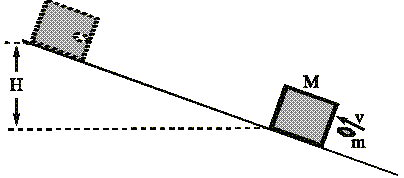
\includegraphics[scale=.6]{/Users/jgates/desktop/latex/pics/inclinebulletblock}
%\end{floatingfigure}
 
{\bf \Large{\arabic{ProbNum}}} A 780 g block is released from rest and slides down a $20^{\circ}$ frictionless incline into a spring attached to a fixed bumper.  The block compresses the spring a maximum distance of 4 cm.  

\bigskip
Determine from how far up the incline (as measured from the tip of the spring) the block was released.\paragraph{}
\noindent
\vfill

\begin{floatingfigure}[r]{.5\textwidth}
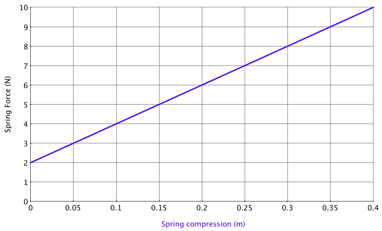
\includegraphics[scale=.75]{/Users/jgates/desktop/latex/pics/springgraph1}
\end{floatingfigure}

The same block is now slid along a level frictionless table with an initial speed of ${2~\tfrac{m}{s}}$.  It hits a spring which does not follow Hooke's law.  The \emph{force vs. compression distance} graph for the spring is shown at right.

\bigskip
Determine the acceleration of the block after it has compressed the spring 5 cm and how fast it is moving at that point.
\vfill
%\hfill 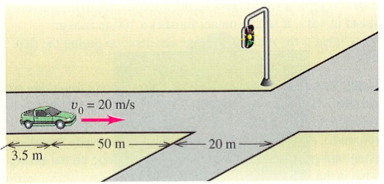
\includegraphics[scale=.85]{/Users/jgates/desktop/latex/pics/redlight.png}
\newpage